%%%%%%%%%%%%%%%%%%%%%%%%%%%%%%%%%%%%%%%%%
% Arsclassica Article
% LaTeX Template
% Version 1.1 (10/6/14)
%
% This template has been downloaded from:
% http://www.LaTeXTemplates.com
%
% Original author:
% Lorenzo Pantieri (http://www.lorenzopantieri.net) with extensive modifications by:
% Vel (vel@latextemplates.com)
% Johan Bos (johan.bos@rug.nl)
% Barbara Plank (bapl@itu.dk)
% 
% License:
% CC BY-NC-SA 3.0 (http://creativecommons.org/licenses/by-nc-sa/3.0/)
%
%%%%%%%%%%%%%%%%%%%%%%%%%%%%%%%%%%%%%%%%%

%-------------------------------------------------------------------
%	PACKAGES AND OTHER DOCUMENT CONFIGURATIONS
%-------------------------------------------------------------------
\documentclass[
10pt, % Main document font size
a4paper, % Paper type
oneside, % One page layout (no page indentation)
headinclude,footinclude, % Extra spacing for the header and footer
%BCOR5mm, % Binding correction
] {book}%
\usepackage{eurosym}
\usepackage{booktabs} % for nice tables with \toprule, \midrule
\usepackage{csvsimple,longtable}
\usepackage{booktabs}
\setcounter{secnumdepth}{5}
%%%%%%%%%%%%%%%%%%%%%%%%%%%%%%%%%%%%%%%%%
% Arsclassica Article
% Structure Specification File
%
% This file has been downloaded from:
% http://www.LaTeXTemplates.com
%
% Original author:
% Lorenzo Pantieri (http://www.lorenzopantieri.net) with extensive modifications by:
% Vel (vel@latextemplates.com)
%
% License:
% CC BY-NC-SA 3.0 (http://creativecommons.org/licenses/by-nc-sa/3.0/)
%
%%%%%%%%%%%%%%%%%%%%%%%%%%%%%%%%%%%%%%%%%

%----------------------------------------------------------------------------------------
%	REQUIRED PACKAGES
%----------------------------------------------------------------------------------------

\usepackage[
%nochapters, % Turn off chapters since this is an article        
beramono, % Use the Bera Mono font for monospaced text (\texttt)
eulermath,% Use the Euler font for mathematics
pdfspacing, % Makes use of pdftex letter spacing capabilities via the microtype package
dottedtoc % Dotted lines leading to the page numbers in the table of contents
]{classicthesis} % The layout is based on the Classic Thesis style


\usepackage{arsclassica} % Modifies the Classic Thesis package

\usepackage[T1]{fontenc} % Use 8-bit encoding that has 256 glyphs

\usepackage[utf8]{inputenc} % Required for including letters with accents

\usepackage{graphicx} % Required for including images

\usepackage{enumitem} % Required for manipulating the whitespace between and within lists

\usepackage{lipsum} % Used for inserting dummy 'Lorem ipsum' text into the template

\usepackage{subfig} % Required for creating figures with multiple parts (subfigures)

\usepackage{amsmath,amssymb,amsthm} % For including math equations, theorems, symbols, etc

\usepackage{varioref} % More descriptive referencing
\usepackage{color}
\usepackage{listings}
\usepackage{setspace}
\usepackage{lscape}
\usepackage[authoryear]{natbib}

%----------------------------------------------------------------------------------------
%	DUTCH SUPPORT
%----------------------------------------------------------------------------------------

%\usepackage[dutch]{babel}    % comment out if you write your thesis in Dutch


%----------------------------------------------------------------------------------------
%	THEOREM STYLES
%---------------------------------------------------------------------------------------

\theoremstyle{definition} % Define theorem styles here based on the definition style (used for definitions and examples)
\newtheorem{definition}{Definition}

\theoremstyle{plain} % Define theorem styles here based on the plain style (used for theorems, lemmas, propositions)
\newtheorem{theorem}{Theorem}

\theoremstyle{remark} % Define theorem styles here based on the remark style (used for remarks and notes)

%----------------------------------------------------------------------------------------
%	HYPERLINKS
%---------------------------------------------------------------------------------------

\hypersetup{
%draft, % Uncomment to remove all links (useful for printing in black and white)
colorlinks=true, breaklinks=true, % bookmarks=true,
bookmarksnumbered,
urlcolor=webbrown, linkcolor=RoyalBlue, citecolor=webgreen, % Link colors
pdftitle={}, % PDF title
pdfauthor={\textcopyright}, % PDF Author
pdfsubject={}, % PDF Subject
pdfkeywords={}, % PDF Keywords
pdfcreator={pdfLaTeX}, % PDF Creator
plainpages=false,
pdfproducer={LaTeX with hyperref and ClassicThesis} % PDF producer
}


\renewcommand{\lstlistingname}{Python code}% Listing -> Python
\renewcommand{\lstlistlistingname}{List of \lstlistingname}% List of Listings -> List of Python
\definecolor{Code}{rgb}{0,0,0}
\definecolor{Decorators}{rgb}{0.5,0.5,0.5}
\definecolor{Numbers}{rgb}{0.5,0,0}
\definecolor{MatchingBrackets}{rgb}{0.25,0.5,0.5}
\definecolor{Keywords}{rgb}{0,0,1}
\definecolor{self}{rgb}{0,0,0}
\definecolor{Strings}{rgb}{0,0.63,0}
\definecolor{Comments}{rgb}{0,0.63,1}
\definecolor{Backquotes}{rgb}{0,0,0}
\definecolor{Classname}{rgb}{0,0,0}
\definecolor{FunctionName}{rgb}{0,0,0}
\definecolor{Operators}{rgb}{0,0,0}
\definecolor{Background}{rgb}{0.98,0.98,0.98}




 
\lstdefinestyle{mystyle}{
numbers=left,
numberstyle=\footnotesize,
numbersep=1em,
xleftmargin=1em,
framextopmargin=10em,
framexbottommargin=2em,
showspaces=false,
showtabs=false,
showstringspaces=false,
frame=l,
tabsize=4,
% Basic
basicstyle=\ttfamily\small\setstretch{1},
backgroundcolor=\color{Background},
language=Python,
% Comments
commentstyle=\color{Comments}\slshape,
% Strings
stringstyle=\color{Strings},
morecomment=[s][\color{Strings}]{"""}{"""},
morecomment=[s][\color{Strings}]{'''}{'''},
% keywords
morekeywords={import,from,class,def,for,while,if,is,in,elif,else,not,and,or,print,break,continue,return,True,False,None,access,as,,del,except,exec,finally,global,import,lambda,pass,print,raise,try,assert},
keywordstyle={\color{Keywords}\bfseries},
% additional keywords
morekeywords={[2]@invariant},
keywordstyle={[2]\color{Decorators}\slshape},
emph={self},
emphstyle={\color{self}\slshape},
captionpos=b, 
}
 
\lstset{style=mystyle}

\def\vl{\\[9pt]}
 % Include the structure.tex file which specified the document structure and layout

\hyphenation{Fortran hy-phen-ation} % Specify custom hyphenation points in words with dashes where you would like hyphenation to occur, or alternatively, don't put any dashes in a word to stop hyphenation altogether

%-----------------------------------------------------------
%	TITLE AND AUTHOR(S)
%-----------------------------------------------------------
\title{\normalfont\spacedallcaps{My Fancy Title}} % The article title
\author{\spacedlowsmallcaps{YOUR NAME HERE}} % The article author(s) - author affiliations need to be specified in the AUTHOR AFFILIATIONS block
\date{} % An optional date to appear under the author(s)

%%%%%%%%%%%%%%%%%%%%%%%%%%%%%%%%%%%%%%%%%
\begin{document}
%\renewcommand{\chaptermark}[1]{\markright{\spacedlowsmallcaps{#1}}} % The header for all pages (oneside) or for even pages (twoside)
%\renewcommand{\subsectionmark}[1]{\markright{\thesubsection~#1}} % Uncomment when using the twoside option - this modifies the header on odd pages
%\lehead{\mbox{\llap{\small\thepage\kern1em\color{halfgray} \vline}\color{halfgray}\hspace{0.5em}\rightmark\hfil}} % The header style
\pagestyle{scrheadings} % Enable the headers specified in this block

%-------------------------------------------------------
%	TITLE PAGE
%-------------------------------------------------------
\hypersetup{pageanchor=false}

\begin{titlepage}
\thispagestyle{empty}
\begin{figure}[h!] %  figure placement: here, top, bottom, or page
\centering

\includegraphics[width=4in]{ITUlogo} 
\end{figure}

\begin{center}
\vspace{30 mm}
\begingroup \linespread{1,75} \selectfont 
\textsc{\LARGE Fancy Title}\\
% \textsc{\Large And this is an optional subtitle}
[1,5cm]
\endgroup

YOUR NAME HERE\\[2,5cm]

\end{center}
\vfill
\textbf{Bachelor thesis}\\  %\textbf{Master thesis}\\
Data Science\\  
Your Name here\\
\\
\today\\
Supervisor: Stella Graßhof
\end{titlepage}

\hypersetup{pageanchor=true}

%------------------------------------------------------
%	ABSTRACT
%------------------------------------------------------
\pagenumbering{roman}
\chapter*{Abstract}
\markboth{Abstract}{Abstract}
\addcontentsline{toc}{chapter}{Abstract}

Short version of my work

%-------------------------------------------------------
%	TABLE OF CONTENTS & LISTS OF FIGURES AND TABLES
%-------------------------------------------------------
\clearpage
\setcounter{tocdepth}{3} % Set the depth of the table of contents to show sections and subsections only
\tableofcontents % Print the table of contents
%\listoffigures % Print the list of figures (optional, only if you have many figures)
%\listoftables % Print the list of tables (optional, only if you have many tables)
%\lstlistoflistings

%%%%%%%%%%%%%%%%%%
% \chapter*{Preface}
% \markboth{Preface}{Preface}
% \addcontentsline{toc}{chapter}{Preface}

%%%%%%%%%%%%%%%%%%%%%%%%%%%%%%%%%%%%%%%
\pagenumbering{arabic}
% introduction.tex
\chapter{Introduction}

In Fig.~\ref{fig:dummy} ...

This concept is explained in \cite{langid}.

\begin{figure}[tb] 
    \centering
    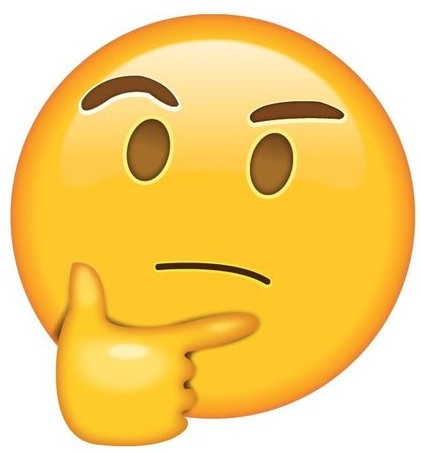
\includegraphics[width=0.3\textwidth]{figs/dummy_img.jpg}
    \caption{This image was published before \cite{fer}.}
    \label{fig:dummy}
\end{figure}

\section{Related Work}


The work is structured as follows 


\chapter{Methods}
\label{ch:methods}

describe all tools which you use


\section{Fancy Statistical Test Procedure}


 

\chapter{Datasets}
\label{ch:data}


\section{Dataset 1}
\label{sec:data1}

The Dataset 1 \cite{wiki} contains 100 persons \ldots 
In Fig.~\ref{fig:data1} four examples are illustrated:
In Fig.~\ref{fig:data1}\subref{subfig:data1_p1} person 1 smiles \ldots 

\begin{figure}[htb]
    \centering
    %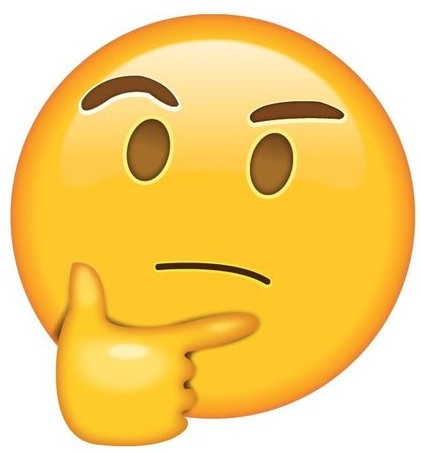
\includegraphics[width=0.3\textwidth]{figs/dummy_img}
    \subfloat[person 1 ]{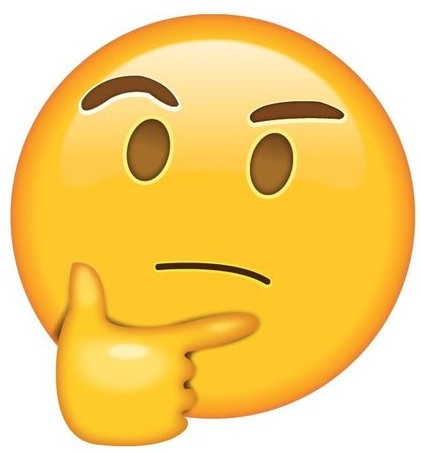
\includegraphics[width=0.24\textwidth]{figs/dummy_img}\label{subfig:data1_p1}}
    \subfloat[person 2 ]{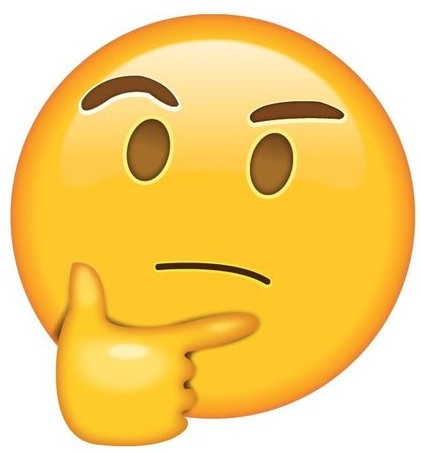
\includegraphics[width=0.24\textwidth]{figs/dummy_img}\label{subfig:data1_p2}}
    \subfloat[person 3 ]{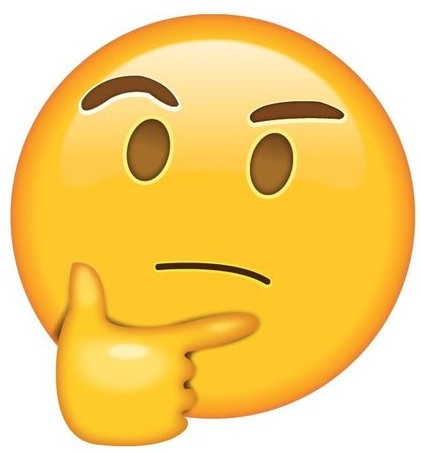
\includegraphics[width=0.24\textwidth]{figs/dummy_img}\label{subfig:data1_p3}}\\
    \subfloat[person 4 ]{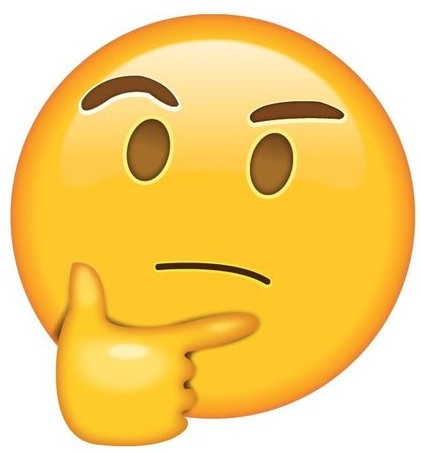
\includegraphics[width=0.24\textwidth]{figs/dummy_img}\label{subfig:data1_p4}}\\

    \caption{Samples from Dataname, with varying persons: \protect\subref{subfig:data1_p1}: smile, \protect\subref{subfig:data1_p2} person 2 frowns,  \protect\subref{subfig:data1_p3} shows Tom Hanks, \protect\subref{subfig:data1_p4} fancy stuff.}
    \label{fig:dataset1}
\end{figure}



\chapter{Experiments}

In this chapter \ldots 

\section{Quantitative Quality Measures}
\label{sec:measures}
\textcolor{red}{THIS SECTION COULD ALSO BE IN THE METHODS CHAPTER}

example equation
\begin{align}
    MSE(a,b) &= \frac{1}{N}\sum_{n=1}^N||a_n-b_n||_2^2
    \label{eq:mse}
\end{align}
% % features, model, evaluation


\section{Classification X}
\textcolor{red}{EXAMPLES FOR REFERENCES AND CITATION OF CODE: ADD ENTRIES TO references.bib} 
The model described in Sec.~\ref{sec:model_age}... 

implementation is based on \cite{vgg_github_2020}, which was combined with \cite{lia_corrales_2015_15991}. 

measure for evaluation Sec.~\ref{sec:measures}, MSE \eqref{eq:mse}

\section{Group Analysis}

In Fig.~\ref{fig:subfigs} it can be seen \ldots 
Fig.~\ref{fig:subfigs}\subref{subfig:input} the original image, \ldots Fig.~\ref{fig:subfigs}\subref{subfig:detect} \ldots 

\begin{figure}[htb] % "H"ere, "T"op "B"ottom
    \centering
    \subfloat[original]{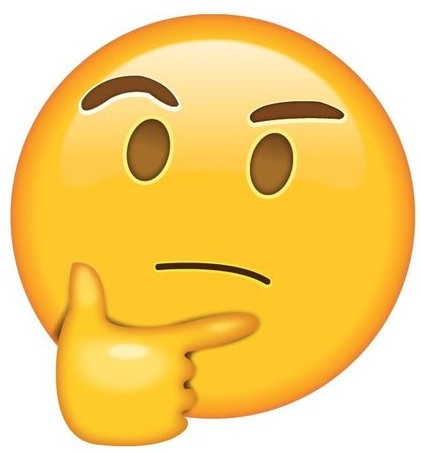
\includegraphics[width=0.3\textwidth]{figs/dummy_img} \label{subfig:input}}
    \subfloat[detected]{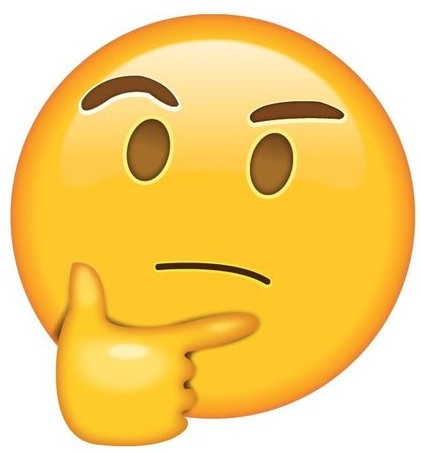
\includegraphics[width=0.25\textwidth]{figs/dummy_img} \label{subfig:detect}}
    \\ % new line if needed
    \subfloat[example 2]{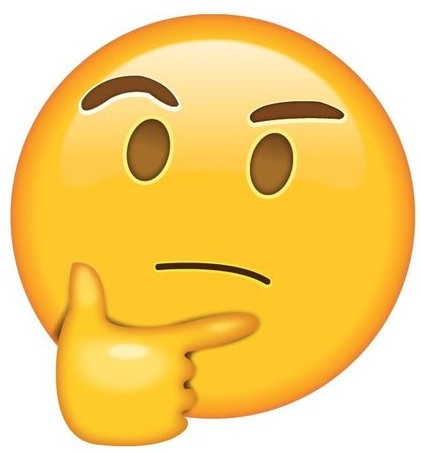
\includegraphics[width=0.48\textwidth]{figs/dummy_img}}
    \subfloat[estimated]{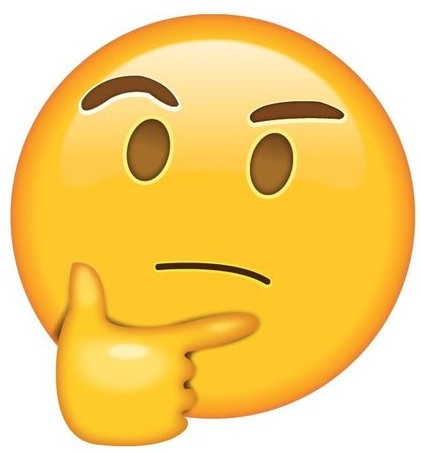
\includegraphics[width=0.48\textwidth]{figs/dummy_img} \label{subfig:ex2}}
    \caption{%
    There should be a short description here. More details in the text: \protect\subref{subfig:input} original image, \protect\subref{subfig:detect} 
    \textcolor{red}{2DO: adapt content, size and description. You can put it all in one row, too.}
    }
    \label{fig:subfigs}
\end{figure}





\chapter{Results and Discussion}
\textcolor{red}{THIS FILE IS MAYBE NOT NEEDED}

Results and Discussion could also be two separate chapters. 

\begin{table}[htb]
    \centering
    \begin{tabular}{cc}
    \toprule 
         M1 & M2 \\ \midrule
       0.5  & \textbf{0}\\
        0.2 &  2\\
     \bottomrule
    \end{tabular}
    \caption{Caption}
    \label{tab:mse_results}
\end{table}

\chapter{Conclusion}
\label{ch:conclusion}

conclude and restate main finding, answer research question

point to limitations and future work

\section{Limitations}
As our study was limited in the time and resources available, it is far from conclusive. We will describe a few of its limitations below.


\chapter{Future Work}

%--------------------------------------------------------------
%	BIBLIOGRAPHY
%--------------------------------------------------------------
%\bibliographystyle{chicago} % from template
% I prefer the following ones
\bibliographystyle{abbrv} 
%\bibliographystyle{plain}  
\bibliography{references}

%--------------------------------------------------------------
%	APPENDICES
%--------------------------------------------------------------
\newpage
\appendix
\chapter{Appendix}
IF YOU LIKE TO HAVE IT

\end{document}
